\subsection{Developers using AdaptUI}
\label{sec:developers}

Before introducing the results obtained from working with potential final users
of AdaptUI (as consumers of adapted user interfaces), an experiment has been
carried out involving developers with previous experience with Android development.
This experiment aims to evaluate the provided \acp{api} and to compare the 
differences between performing a configuration of the user interface in Android
and in AdaptUI. 

As AdaptUI provides two different \acp{api}, this experiment has been divided
in two parts. The first one deals with the adaptation \ac{api}. This \ac{api}
aims to ease the adaptation process by calling several methods related to the
aspect of the different elements displayed on the screen. The second part's goal
is to show developers how to modify the knowledge of the AdaptUIOnt ontology.

\subsubsection{The adaptation \ac{api}}
\label{sec:adaptation_api}

The adaptation \ac{api} provide a set of methods with purpose of easing the 
adaptation process for developers. As previous Android development experience
is needed, the idea of this \ac{api} is to maintain the design paradigm established
by Android. This includes layout configuration \ac{xml} file, in which the 
declaration of the user interface elements have to be detailed; and also a
search and a declaration of the same items in the \textit{onCreate} main method
if any actions are planned with these items (e.g., change their behaviour or
colour).

Listing~\ref{lst:default_layout} shows the Android \ac{xml} layout for the current
experiment, including a grid layout, an edit text, a button and a text view. The
resulting user interface is shown in Figure~\ref{fig:default_layout}.

\inputminted[linenos=true, fontsize=\footnotesize, frame=lines]{xml}{5_experiments_and_results/default_layout.xml}
\captionof{listing}{The default layout defining a grid layout, a text view,
a button and an edit text.\label{lst:default_layout}}

\begin{figure}
\centering
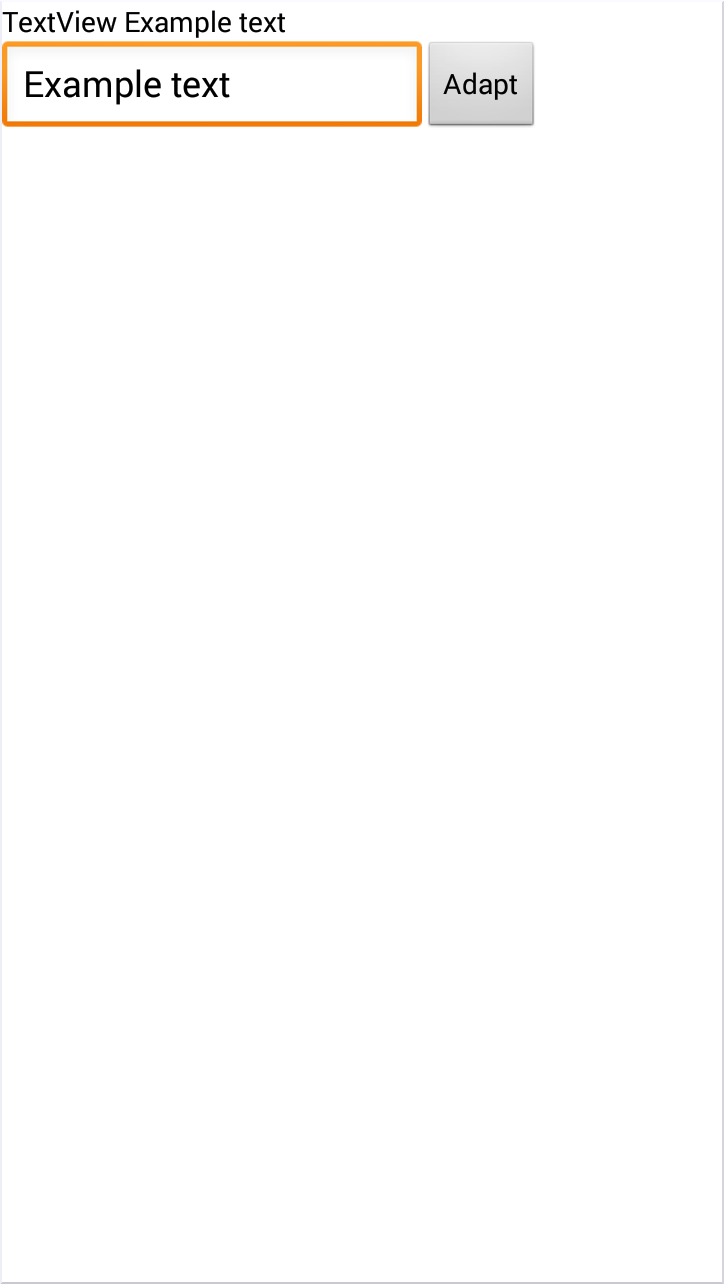
\includegraphics[width=0.35\textwidth]{default_layout.png}
\caption{The corresponding user interface considering the layout specified in
Listing~\ref{lst:default_layout}.}
\label{fig:default_layout}
\end{figure}

The usual Android code for managing the user interface is shown in Listing~\ref{lst:default_oncreate}.
On the contrary, managing dynamic adaptive user interface views is allowed thanks
to the AdaptUI adaptation \ac{api} provided methods. An example is shown in
Listing~\ref{lst:adaptui_oncreate}. In it, it is shown how declaring an \textit{AdaptUI}
object the adaptation of the views is easy and dynamic.


\inputminted[linenos=true, fontsize=\footnotesize, frame=lines]{java}{5_experiments_and_results/default_oncreate.java}
\captionof{listing}{The default \textit{onCreate} method.\label{lst:default_oncreate}}

\inputminted[linenos=true, fontsize=\footnotesize, frame=lines]{java}{5_experiments_and_results/adaptui_oncreate.java}
\captionof{listing}{The AdaptUI \textit{onCreate} method.\label{lst:adaptui_oncreate}}

\subsubsection{The knowledge editor \ac{api}}
\label{sec:knowledge_api}